\documentclass[conference]{IEEEtran}
\IEEEoverridecommandlockouts

% Packages
\usepackage{cite}
\usepackage{amsmath,amsfonts}
\usepackage{algorithm}
\usepackage{algpseudocode}
\usepackage{graphicx}
\usepackage{textcomp}
\usepackage{xcolor}
\usepackage{booktabs}
\usepackage{adjustbox}
\usepackage{listings}

\usepackage{verbatim}
\usepackage{multirow}

\def\BibTeX{{\rm B\kern-.05em{\sc i\kern-.025em b}\kern-.08em
    T\kern-.1667em\lower.7ex\hbox{E}\kern-.125emX}}

\begin{document}

\title{Deliverable report \\
\footnotesize \textit{"Vittorio Polci": Mat: 257817, \texttt{vittorio.polci@unitn.it}, GitRepo: \texttt{https://github.com/vittorio01/GPU-Computing-2025-257817}}}

\maketitle

\begin{abstract}
The algorithm of sparse matrix-dense vector multiplication (SpMV) is an optimized version of the traditional matrix-vector multiplication, 
designed to handle cases where the matrix is organized in a low density of non-zero entries. 
This technique is particularly useful in scenarios involving very large matrices with a small amount of not null terms because it allows to reduce the used space for 
storing that large structures and, at the same time, optimizes memory accesses and reduces overhead during computational steps. 

This deliverable discusses about the implementation of different parallel implementation of the SpVM algorithm between CSR matrices and a general vector,
with a final benchmark, which evaluates all solution toghether in order to identify the algorithm with the best behaviour. 

\end{abstract}

\begin{IEEEkeywords}
Sparse Matrix, SpMV, CUDA, Parallelization, Storage Format
\end{IEEEkeywords}

\section{Introduction}
The main objective, when developing algorithms that elaborates large quantities of data, is to obtain a solution that:
\begin{enumerate}
    \item Minimizes the execution time. 
    \item Minimizes the memory accesses during the computation of results.
    \item Maintain as much as possible the performance with different inputs. 
\end{enumerate}
Because the SpMV multiplication should handle matrices with millions or billions of not null elements, to obtain good results is necessary to use parallelization techniques 
on GPUs rather than sequential solution for CPUs. 

\section{Problem Statement}
In the SpVM multiplication we consider a matrix coded in a sparse format (in this case the CSR format) and an input vector that has the same size of its columns number. 

Each elements of the resulting vector is computed by summing toghether the dot products of each row of the matrix with the input vector.
\begin{algorithm}[h!]
    \caption{Algorithm for a standard matrix-vector product}
    \begin{algorithmic}[1]
    \Procedure{Function}{$matrix$, $vector$, $output$}
    \For{$row$ in $matrix.rows$}
    \For{$element$ in $row$}
    \State $output[row]$
    \State $= input[element]*output[element]$
    \EndFor
    \EndFor
    \EndProcedure
    \end{algorithmic}
\end{algorithm}
At this point the main objectives are:
\begin{enumerate}
    \item Create a first sequential algorithm that performs the same operation on a sparse CSR matrix.
    \item Parallelize in different ways the first CPU implementation with CUDA and compare them in terms of performances and resurces utilization. 
\end{enumerate}

\subsection{Storage Format}
The CSR for sparse matrices is a storage format that involves three different arrays to represent the information: 
\begin{itemize}
    \item The data array, that contains all not null terms of the original matrix.
    \item The column array, that for each element in the data vector specifies its column coordinate. For example, the element $i$ in the data array has its respective column coordinate stored in $colArray[i]$
    \item The row array, which contains the start and the end pointers for each row to the data and column arrays. these two pair of pointers indicates which data are contained in that specific row. 
\end{itemize}
At the end, the size of the data and column arrays depends on the number of not null elements and the size of the row array depends on the number of the rows in the original matrix. 
\begin{figure}[H]
    \centering
    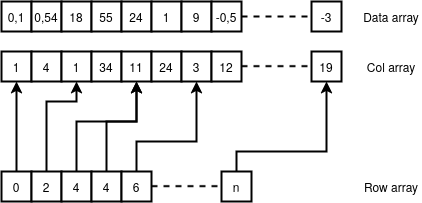
\includegraphics[width=0.8\linewidth]{images/CSR.png}
    \caption{Data organization in CSR structure}
    \label{fig:csr-format}
\end{figure}
For example, all elements in contained in a row $i$ are enumerated in the data array starting from the position stored in the row array $rowArray[i]$ to the position stored in the next cell $rowArray[i+1]$.

\subsection{Parallelization}
To improve the overall performance, the parallel implementation of the first algorithm are designed to be executed on Nvidia GPUs and programmed in CUDA.
The CUDA language model is designed to run on different concurrent threads called CUDA cores, where each thread represents a computational unit located in the GPU. 

In general, the workload can be splitted in different ways for a certain number of CUDA cores. Different organizations can provide more or less performance in terms of the execution time and 
troughput. 

\section{State of the Art}
There already are multiple c++ libraries that performs CSR SpMV multiplications:
\begin{itemize}
    \item cuSPARSE\cite{cuSPARSE}, the official library supported by Nvidia that can perform multiplication between matrices and vectors in different formats with CUDA. 
    \item MAGMA-sparse\cite{magma}, a linear algebra library that offers solution for multicore/multithreads algorithms that runs on CPUs and GPUs. 
    \item Ginkgo\cite{ginkgo}, like MAGMA offers high-performance solution for multicore linear algebra algorithms for different platforms.
\end{itemize}
All listed libraries includes also shared memory optimizations, pipelining and other techniques to improve the performance of the algorithm. 

The proposed algorithms in this derivable includes solutions that designed to performs only in the GPU's global memory. 


\section{Methodology and Contributions}\label{sec:methodology}
\subsection{Sequential algorithm}
There are not so much solutions to implement a sequential SpVM multiplication. The most intuitive and performant way is to scan the row vector and, using the 
stores pointers, perform the product and accumulate over a variable all the elements contained in each row.

\begin{algorithm}[h!]
\caption{Sequential version for the SpVM algorithm}
\algorithmicrequire~The input matrix structure $matrix$ that contains all arrays and sizes, the input vector $input$ structure, the number of not null elements $notNull$), the input vector structure (that contains the data array $dataArray$) and the output vector $output$ structure.
\begin{algorithmic}[1]
\Procedure{vmcsrMul}{$output$, $matrix$, $input$}
\For{$i$ in $matrix.rowSize$}
\State $startRow=matrix.rowArray[i]$
\State $endRow=matrix.rowArray[i+1]$
\State $acc=0$
\For{$j$ in ${startRow,\dots,endRow}$}
\State $col=matrix.colArray[j]$
\State $acc+=$
\State $matrix.dataArray[j]*input.dataArray[col]$
\EndFor
\State $output.dataArray[i]=acc$
\EndFor
\EndProcedure
\end{algorithmic}
\label{alg:sequential}
\end{algorithm}
The algorithm \ref{alg:sequential} scans and decodes each pair of start and end pointes for the data array and the column array of the input matrix. 
Using these two values a second loop first decode the column coordinate of each element in the specific row and then computes the product between the corresponding matrix and vector elements and accumulates the result in a value $acc$. 
After a row is processed by the second loop, the accumulated value is then stored in the second vector.

The memory access pattern of this solution permits coalescent accesses in all three arrays of the sparse matrix. The only aspect that limits the performance of the algorithm is that the accesses that gathers the input row elements depends on the values stored in the column array and they cannot be optimized without introducing overhead.
input array should be readed,

\subsection{First parallel implementation}
A first parallel implementation of the algorithm \ref{alg:sequential} divides the workload between threads such a way that each thread processes one or more entire rows

The first operation that the algorithm performs is divide the workload for each thread. In particular:
\begin{enumerate}
    \item The row array is splitted in equal subsection that will be assigned to different blocks of threads using the ceiling division system. 
    \item The obtained subsection are then divided in the same way in order to assign equal workload to each thread.
\end{enumerate}
\begin{figure}[H]
    \centering
    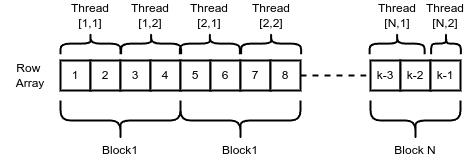
\includegraphics[width=1\linewidth]{images/ceiling_division.png}
    \caption{Example of workload division for the first parallel implementation (N blocks of 2 threads)}
    \label{fig:ceiling1}
\end{figure}
After that procedure, each thread has his number of row to process $rowsPerThread$, the start position $threadStart$ and the end position $threadEnd$ in the row array.
\begin{algorithm}[h!]
\caption{First parallelization for the SpVM algorithm}
\algorithmicrequire~Same requirements in the sequential implementation but with all structures loaded in the global memory.
\begin{algorithmic}[1]
\Procedure{vmcsrMul}{$output$, $matrix$, $input$}
\State $threadStart,threadEnd$ \Comment{Ceiling division process}
\For{$row$ in ${threadStart,\dots,threadEnd}$}
\State $startRow=matrix.rowArray[i]$
\State $endRow=matrix.rowArray[i+1]$
\State $acc=0$
\For{$j$ in ${startRow,\dots,endRow}$}
\State $col=matrix.colArray[j]$
\State $acc+=$
\State $matrix.dataArray[j]*input.dataArray[col]$
\EndFor
\State $output.dataArray[row]=acc$
\EndFor
\EndProcedure
\end{algorithmic}
\label{alg:parallel1}
\end{algorithm}

The algorithm \ref{alg:parallel1} is the simplest implementation and has good performances for common sparse matrices because:
\begin{itemize}
    \item For each thread the accesses are coalescent in all arrays of the matrix.
    \item Each thread works on the single rows independently and there is not concurrency at all. 
\end{itemize}


\subsection{Second parallel implementation}
One problem of the algorithm \ref{alg:parallel1} is that if there are threads that have much more more workload to perform, the computational time 
might be affected negatively. This is the case for matrices which have consecutive rows that contains much more not null elements compared to the others.

A solution that may mitigate this problem is to use a dynamic assignment of the rows to threads that are in the same block:
\begin{enumerate}
    \item The row array is splitted in equal subsection for different blocks using again the ceiling division. 
    \item For each block a variable in the shared memory $pendingRow$ corresponds to the next row that is waiting for the assignment. 
    \item Each thread uses the function $atomicAdd(pendingRow,1)$ to increment the value of $pendingRow$ and, at the same time, read its content
    and computes the corresponding row until they reach the end of their subsection. 
\end{enumerate}

\begin{algorithm}[h!]
\caption{Second parallelization for the SpVM algorithm}
\algorithmicrequire~Same requirements as the algorithm \ref{alg:parallel1}.
\begin{algorithmic}[1]
\Procedure{vmcsrMul}{$output$, $matrix$, $input$}
\State $blockStart,blockEnd$ \Comment{Ceiling division}
\State $pendingRow=0$ \Comment(only thread 0);
\State $syncthreads()$
\While {${true}$}
\State $pendingRow=atomicAdd(pendingRow,1)$
\State $+blockStart$
\If {$pendingRow>blockEnd$} \Return \EndIf
\State $startRow=matrix.rowArray[pendingRow]$
\State $endRow=matrix.rowArray[pendingRow+1]$
\State $acc=0$
\For{$j$ in ${startRow,\dots,endRow}$}
\State $col=matrix.colArray[j]$
\State $acc+=$
\State $matrix.dataArray[j]*input.dataArray[col]$
\EndFor
\State $output.dataArray[pendingRow]=acc$
\EndWhile
\EndProcedure
\end{algorithmic}
\label{alg:parallel2}
\end{algorithm}

The dynamic assignment for threads in the same block implemented in the algorithm \ref{alg:parallel2} tries to mitigate the unbalanced workload introduced in some rows. 
In facts, if some thread spend too much time when computing a single row, other available threads may perform also rows that in the algorithm \ref{alg:parallel1} should be reserved for others.  
Two limitation introduced with this system are:
\begin{itemize}
    \item There is concurrency for the value $pendingRow$ that may limit the performance. 
    \item There is a large probability that some threads do not elaborate rows that are coalescent in the matrix arrays. 
\end{itemize}

\subsection{Third parallel implementation}
Another tentative to distribute the workload contained in the single rows is to parallelize the algorithm such that each row is assigned to 
single blocks instead of threads:
\begin{enumerate}
    \item The row array is splitted for different blocks as usual. 
    \item For each row all threads does some multiplication (or not) of a certain number of elements and accumulates the result in the output vector using the function $atomicAdd()$. 
\end{enumerate}

\begin{algorithm}[h!]
\caption{Second parallelization for the SpVM algorithm}
\algorithmicrequire~Same requirements as the algorithm \ref{alg:parallel1}.
\begin{algorithmic}[1]
\Procedure{vmcsrMul}{$output$, $matrix$, $input$}
\State $blockStart,blockEnd$ \Comment{Ceiling division}
\For{$row$ in ${blockStart,\dots,blockEnd}$}
\State $startRow=matrix.rowArray[row]$
\State $endRow=matrix.rowArray[row+1]$
\State $elements=endRow-startRow$
\If{$elements<blockSize.x$}
\State $col=matrix.colArray[j]$
\State $atomicAdd($
\State $output.dataArray[row],$
\State $matrix.dataArray[threadIdx.x]*$
\State $input.dataArray[col]$
\State $)$
\Else 
\State $threadStart,$
\State $threadEnd$ \Comment {Ceiling division on row}
\State $acc=0$
\For{$j$ in ${threadStart,\dots,threadEnd}$}
\State $col=matrix.colArray[j]$
\State $acc+=matrix.dataArray[j]*$
\State $input.dataArray[col]$
\EndFor
\State $atomicAdd($
\State $output.dataArray[row],acc$
\State $)$
\EndIf
\EndFor
\EndProcedure
\end{algorithmic}
\label{alg:parallel3}
\end{algorithm}

The algorithm \ref{alg:parallel3} distributes the workload of a row on blocks of threads instead single threads but, without using shared memory optimization, this creates more overhead because:
\begin{itemize}
    \item If the block size is large the function $atomicAdd()$ creates a barrier that limits too much the performance because it must guarantee atomic accumulation on the output vector. 
    \item The first threads in a block are overused for all rows but the last threads are used only if the number of rows are large enough to require them. 
\end{itemize}

\section{System Description and Experimental Set-up}
\subsection{Dataset description}
A dataset composed by 6 matrices is used for testing and benchmark all four algorithms. These matrices containes a number of not null elements between 1 and 1,5 million of not null elements.
These matrices have different organization of the elements and dispersion that challenges the algorithms in different ways:
\begin{itemize}
    \item Linux\_call\_graph represents one of the worst cases because it has a large amount of not null elements that are distribuited on all original matrix.
    \item Nemeth24 represents one of the better cases because it has a low amount of elements that are concentrated on the diagonal.
\end{itemize}
The used dataset is obtained from the SuiteSparse Matrix Collection \cite{suitesparse}, a website that contains sample matrices which can be used for benchmarking algorithms. 

\begin{table}[h]
    \centering
    \begin{adjustbox}{width=\columnwidth}
    \begin{tabular}{llllrl}
    \toprule
    \textbf{Dataset} & \textbf{Dimension (R x C)} & \textbf{Non-zero entries} & \textbf{Type} \\
    \midrule
    dbir2 \cite{dbir2} & 18,906 x 45,887 & 1,158,159 & Unbalanced rows \\
    ex11 \cite{ex11} & 16,614 x 16,614 & 1,096,948  & Diagonally distributed (low density) \\
    language \cite{language} & 399,130 x 199,130 & 1,216,334 & Upper triangular \\
    Linux\_call\_graph \cite{linuxcallgraph} & 324,085 x 324,085 & 1,208,908 & Dense matrix (worst case) \\
    nemeth24 \cite{nemeth24} & 9,506 x 9,506 & 1,506,550 & Diagonally distributed (best case) \\
    twotone \cite{twotone} & 120,750 x 120,750 & 1,206,265 & Diagonally distributed (moderate dispersion) \\
    \bottomrule
    \end{tabular}
    \end{adjustbox}
    \vspace{1em}
    \caption{Structural patterns of the benchmark sparse matrices.}
    \label{tab:my_label}
\end{table}

\subsection{System Description}
The system used for the execution of the benchmarks is uses CUDA 12.3.2, GCC 11.5.0, and is composed by a Intel(R) Xeon(R) Silver 4214 CPU and A Nvidia A30 GPU.  

\begin{table}[h]
    \centering
    \begin{adjustbox}{width=\columnwidth}
    \begin{tabular}{lll}
    \toprule
    \textbf{Characteristic} & \textbf{Value} & \textbf{Device}\\
    \midrule
    Global memory & 24 GB &  \multirow{5}{*}{\textbf{GPU: Nvidia A30}} \\
    Theoretical BW & 933 GB/s \\
    CUDA Cores & 10752 \\
    SM Number & 108 \\
    FP32 Performance & 10.3 TFLOPS \\
    \midrule 
    Cores number & 12 & \multirow{3}{*}{\textbf{CPU: Intel(R) Xeon(R) Silver 4214}} \\
    Threads number & 24 \\
    Clock speed & 2.2Ghz \\
    \bottomrule
    \end{tabular}
    \end{adjustbox}
    \vspace{1em}
    \caption{Benchmark system specs}
    \label{tab:benchmarkSystem}
\end{table}

\subsection{Experimental Set-up}
The performance is measured using the execution time elapsed measured with the C function $getTimeOfDay()$ for the sequential algorithm and $cudaEventRecord$ functions for CUDA algorithms. 

Each algorithm is executed 25 times (5 warmup cycles and 20 iterations) and from the execution times (in milliseconds) is performed the geometric mean to remove eventual outlayers. 

From the average execution time is then performed the effective bandwidth and the FLOP/s.

\begin{equation}
effBW (GB/s)=\frac{readedBytes+writtenBytes}{executionTime(ms)}*10^{-6}
\end{equation}

\begin{equation}
GFLOPS/s= \frac{floatingPointOp}{executionTime(ms)}*10^{-6}
\end{equation}

\section{Experimental Results}
Present and discuss results. Include plots and tables when required (like Figure \ref{fig:enter-label}). Do not simply describe the figures; criticise the achieved results by underlining how they confirm/differ from the expected outcomes described in Section \ref{sec:methodology}.

\begin{figure}[H]
    \centering
    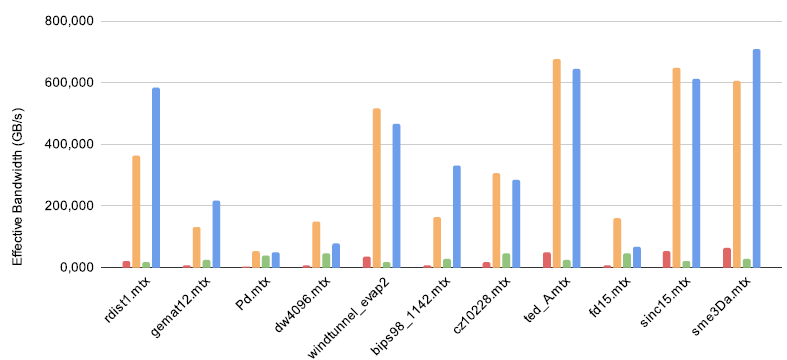
\includegraphics[width=0.95\linewidth]{SampleImage.png}
    \caption{Caption}
    \label{fig:enter-label}
\end{figure}

\section{Conclusions}
[max 200 words]\\
Summarize findings and future work \dots
\bibliographystyle{IEEEtran}
\bibliography{references}

\end{document}

